\epigraph{Well, my theory is that your theory is wrong.}{Fernanda G. P. Susemihl}

In the previous chapter I have introduced filtering methods for stochastic processes observed through Poisson processes. In this chapter I will deal with the issue of how well one
can estimate that process from a set of Poisson processes with a given set of rate functions.\par

If one has an estimate $\hat{X}$ of some stochastic variable $X$ to be estimated , how
can one quantify the error incurred by the estimator? One needs to specify some loss function that assigns a cost to an error $|\hat{X}-X|$. It makes sense to require the loss function to
be increasing and to require the loss of an exact estimate to be zero, but other than that, any loss function could do. Here I will consider results on the squared loss function
\[
L^2(\hat{X},X) = (\hat{X}-X)^2,
\]
leading to the mean-squared-error (MSE) as a measure of the performance of the encoder. This is specially convenient when dealing with Gaussian distributions, as a number of 
analytical  results can be derived. Other possible choice would be the absolute loss, given by
\[
L^1(\hat{X},X) = |\hat{X}-X|.
\]
In other situations, such as classification tasks, other loss functions are useful, but I will restrict myself to the MSE case here.\par

When dealing with stochastic processes, it is usually more convenient to consider the covariance matrix of the process, rather than the squared error, which is given by the
sum of the variances of every coordinate of the process.
Let me then define the mean-squared error matrix as
\[
\boldsymbol{MSE}(\hat{X}) = \boldsymbol{E}\left[ (\hat{X} - X) (\hat{X}-X)^\top\right],
\]
where the expectation is over all possible realisations of $X$ and over the observations leading to the estimator $\hat{X}$. Alternatively one could take the average to be over
multiple realisations of an experiment, or over long time averages of a temporal estimation problem.
To obtain a scalar measure of the estimation error, one can just take the trace of the MSE matrix.
This scalar error will be written as 
\[
MSE = \Tr( \boldsymbol{MSE}) = \boldsymbol{E}\left[ (\hat{X} - X)^\top (\hat{X}-X)\right].
\]
If further one knows that the estimator $\hat{X}$ depends on some 
parameters $\theta$, she could seek out the optimal estimator $\hat{X}^*$ by taking the parameters $\theta^*$ that minimise the MSE
\[
\theta^* = \textrm{argmin}_\theta MSE( \hat{X}(\theta)  ).
\]
Assuming I am estimating $X$ from an observation process $Y$ dependent on $X$, I can write
\begin{equation}
\label{eq:bayes_mse}
MSE( \hat{X}(Y) ) = \int dX dY  (\hat{X}(Y) - X)^\top (\hat{X}(Y)-X) P(X|Y)P(Y).
\end{equation}
Since $P(Y)\ge 0$ for every $Y$, minimising the inner integrand $\int dX (\hat{X}(Y) - X)^\top (\hat{X}(Y)-X) P(X|Y)$ for every $Y$ will lead to a minimum of the full integral. So, minimising the inner integrand with respect to the estimator will lead to
\[
\frac{\partial \int dX (\hat{X}(Y) - X)^\top (\hat{X}(Y)-X) P(X|Y)}{\partial \hat{X}(Y)} = 2 \int dX (\hat{X}(Y) - X) P(X|Y).
\]
Equating the derivative to zero leads to the minimum mean squared-error (MMSE) estimator for $X$, given by
\[
\hat{X}^*(Y) = \int dX\, X\, P(X|Y) = \boldsymbol{E}[X|Y].
\]
The MMSE estimator is often called the Bayes estimator for $X$ given the observations $Y$, since it minimises an expected loss given by \fref{eq:bayes_mse}, which treats
the quantity being estimated as a random variable with a prior probability distribution.
The MMSE estimator, however, can only be exactly computed if the true data generating distribution $P(Y|X)$ along with the true signal distribution $P(X)$ is known, allowing one
to estimate the posterior probability $P(X|Y)$. Furthermore, the Bayes 
estimator involves averaging over the signal space, which can be impractical. A number of techniques can be used to approximate the estimator though, such as Gaussian
processes or neural networks. The optimality of the MMSE estimator is a central result in information theory, and the MMSE estimator is usually taken as the standard to 
estimation.\footnote{Minimising a different loss function or error measure would lead to a different optimal estimator. Minimising the expected absolute loss, for example, 
leads to the posterior median as the optimal estimator.}
\par

However, finding the optimal estimator is not the end of the story. Often the design of sensors and of the experimental process allow one to change the data 
generating distribution $P(Y|X)$. For a simple example, consider a radar gun. Assume it gives a measure of the speed of the considered vehicle corrupted  with 
Gaussian noise with zero mean and standard deviation of $5\,\textrm{km/h}$. Indeed, given a number of measurements of the speed of a 
vehicle,\footnote{Assuming the speed of the vehicle remained unchanged across measurement} the MMSE estimator will be the estimator which minimises the 
expected 
MSE. Regardless of that, however, one can always reduce the MSE by using a radar gun with a smaller noise rate. A superior radar gun which outputs 
measurements with standard deviation of $1\,\textrm{km/h}$ will certainly reduce the MSE further. In most simple cases, however, this reduction is obvious, as one 
simply strives to reduce the noise as much as possible.
\par

The neural case poses an interesting exception though. Considering the Poisson model from the previous chapter, the probability of a spike being fired in a small time 
interval $dt$ conditioned on the stimulus $X$ is given by $\lambda(X)dt$. The probability of a spike being fired averaged over all stimuli $X$ would then be given by
$\hat{\lambda}dt = \int dx\, P(x)\, \lambda(x)dt$. If one tries to increase the precision of the likelihood defined by $\lambda(X)$, for example by reducing the 
width of the tuning function, this will automatically reduce the probability of that neuron firing. Therefore, there is a trade-off between frequency of firing and precision of 
firing, which is not present in the case of additive Gaussian noise. This is illustrated in \fref{fig:neuron_example}, where I show two Poisson neurons with Gaussian tuning functions
and the same preferred stimulus but with different precisions. The upper neuron has a broader tuning function, leading to a higher firing rate, but in turn the spikes are less 
discriminating of the value of the stimulus. The second neuron has a much narrower tuning function, leading to more precise observations of the stimulus, but a much lower
spiking frequency. It is not immediately clear which neuron will allow for a better reconstruction of the underlying stimulus, as the influence of the frequency and the precision
of the spikes would have to be pitted against each other.
\par

\begin{figure*}
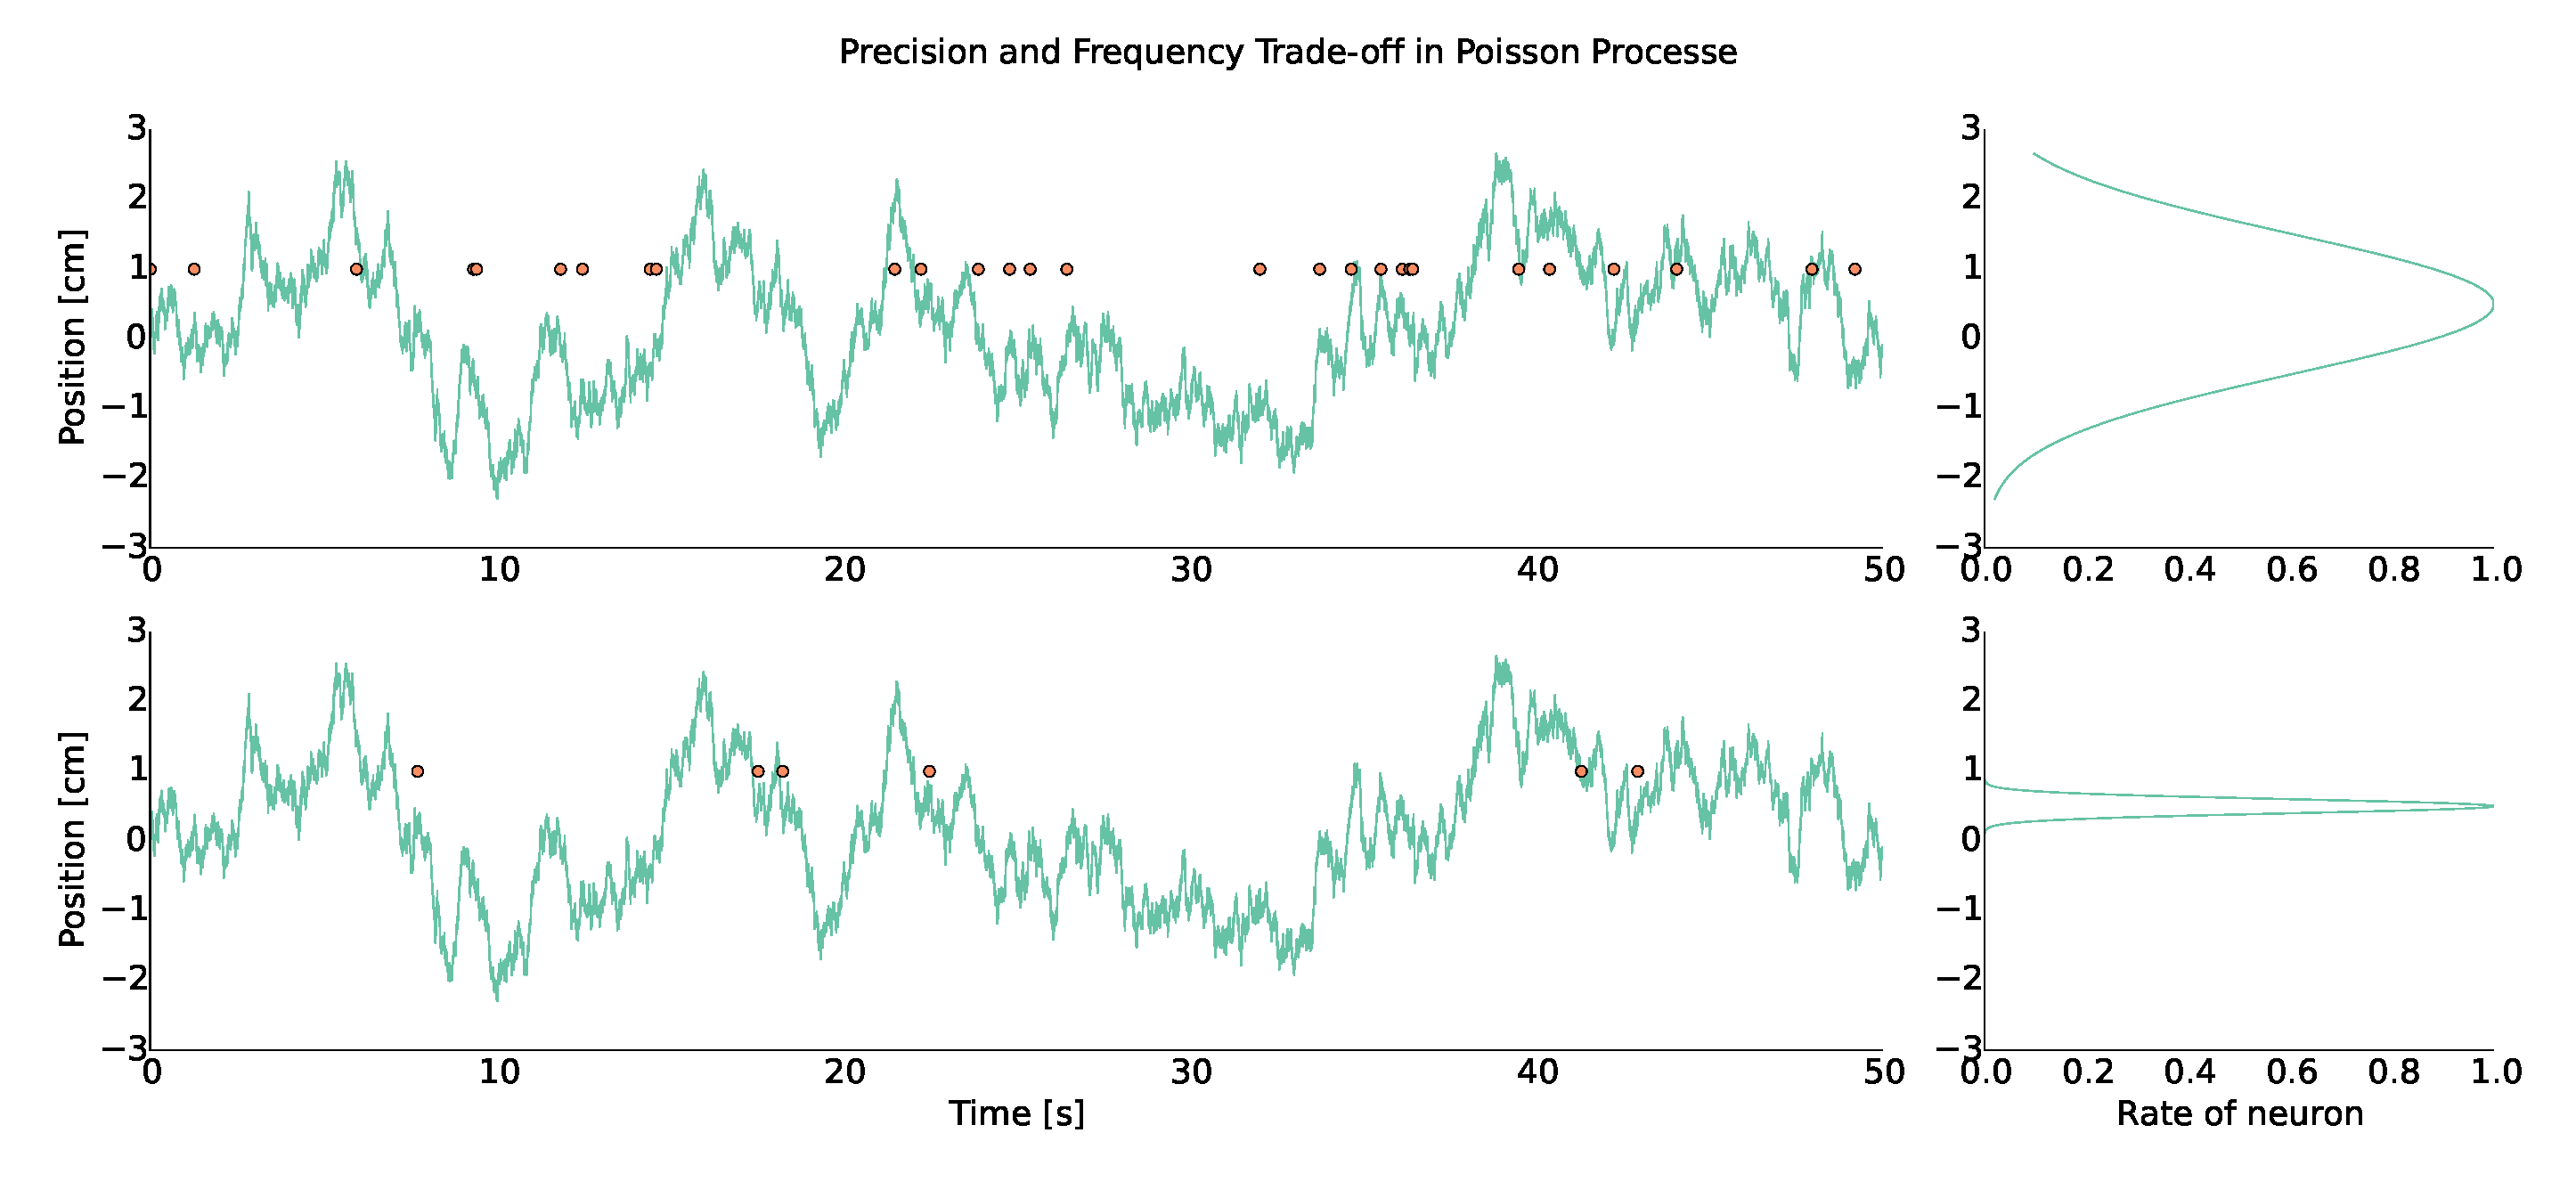
\includegraphics[width=\columnwidth]{figures/figure_3_example.eps}
\caption[Trading off precision and frequency in spike observations.]{The tradeoff between precision and frequency. The upper plot shows the spike train of a single neuron with a Gaussian tuning function with unit width responding to a
stochastic stimulus. There are quite a few spikes but they are fairly unreliable. The lower plot shown a neuron with a Gaussian tuning function with a width of $0.2$. There are
nearly no spikes, but they spike only when the neuron is in a narrow range around the neuron's tuning centre.}
\label{fig:neuron_example}
\end{figure*}

In this chapter I will derive a number of exact and approximate relations for the MSE of the optimal filters described in the previous chapter. I will provide a solution for the stationary distribution of the
posterior variance of the optimal filter for the OU process, showing that this distribution diverges when the average interspike interval is longer than the relaxation time of the variance. I will present a 
number of approximate treatments of limiting cases, for low firing rates and for the diffusion limit of large observation noise. Finally I will provide a treatment of the average posterior
kernel, which allows us to study the MSE of the optimal filter of general Gaussian processes. My goal in this chapter is to develop exact and approximate methods to study the average
MSE performance of the optimal filter of a system observed through a population of doubly stochastic Poisson processes. Armed with that, I will in \fref{chap:optimal} look at the
optimal strategies for these processes to encode the state of system, namely the ones that minimise the MSE.

\section{The MSE for Dense Gaussian DSPP Observations}

In \fref{sec:fast_coding} I have discussed case of dense populations of Gauss-Poisson neurons, first introduced in \mycitep{Huys2007}. 
This framework allows for a number of simplifications. Most importantly, the posterior variance of the filter obeys a SDE with drift and jumps where the jumps occur with
a state-independent rate $\hat{\lambda}$. As I have discussed above, the MMSE estimator gives the optimal estimator for a data-generating distribution $P(Y|X;\covar,\{\theta_i\},\phi)$. 
However, if the response properties of the neural population change (through changes in $\covar$, $\phi$ or the positioning of the tuning functions), the performance of the estimator
will change as well and one can ask which is the encoder that provides the lowest MMSE.
\par

As in \fref{sec:fast_coding}, let the stimulus be a stochastic process $X(t)$, and the observations be spike trains of a dense population of Gauss-Poisson neurons
$\boldsymbol{N}(t) = (N^1(t),\ldots, N^M(t))^\top$. Writing $\boldsymbol{N}_{0:t} = \{\boldsymbol{N}(v), \forall v \in [0,t]\}$, the posterior distribution is
\[
P(X(t)|\boldsymbol{N}_{0:t}) = \mathcal{N} \left(\mu(t;\boldsymbol{N}_{0:t}),\Sigma(t;\boldsymbol{N}_{0:t})\right),
\]
where $\mu(t;\boldsymbol{N}_{0:t})$ and $\Sigma(t;\boldsymbol{N}_{0:t})$ are solutions to \fref{eq:filtering_sdes}.
% with initial conditions $\mu(0) = \mu_0$ and $\Sigma(0)= \Sigma_0$.
The MMSE matrix can be written as
\[
\boldsymbol{MMSE}(t;\{\theta_i\},\covar) = \boldsymbol{E}_{X(t),\boldsymbol{N}_{0:t}}\left[\left(X(t) -\mu(t;\boldsymbol{N}_{0:t})\right)\left(X(t) - \mu(t;\boldsymbol{N}_{0:t})\right)^\top\right]\equiv \epsilon(t).
\]
I am interested in the ensemble average over all possible realisations of both the signal as the observation processes.\par

Throughout this chapter, I assume that the posterior distribution used to evaluate the posterior mean estimator is the same distribution as the one that is generating the observations
$\boldsymbol{N}_{0:t}$. This is called the matched situation. If complete information about the distribution $P(\boldsymbol{N}_{0:t}|X(t))$ was unavailable, one would be forced to work
with an approximate posterior. In the matched case, however, I can simplify the expression for $\epsilon(t)$. Writing out the expectation over $X$ and $\boldsymbol{N}$ gives
\[
\epsilon(t) = \int d\mu\left(X(t)\right) \int d\mu(\boldsymbol{N}_{[0:t]}) \left(X(t) - \mu(t;\boldsymbol{N}_{0:t})\right)\left(X(t) - \mu(t;\boldsymbol{N}_{0:t})\right)^\top P(X| \boldsymbol{N}_{0:t}) P(\boldsymbol{N}_{0:t}).
\]
The average over $P(X|\boldsymbol{N}_{[0:t]})$ will just yield the posterior variance $\Sigma(\boldsymbol{N}_{0:t})$, leading to
\begin{equation}
\label{eq:eps_sigma}
\epsilon(t) = \boldsymbol{E}\left[\Sigma(\boldsymbol{N}_{0:t})\right] = \boldsymbol{E}\left[\Sigma(N_{0:t})\right],
\end{equation}
where in the last step I have used that the posterior variance is only a function of the population spike count $N_{0:t} = \sum_i N^i_{0:t}$ and not of the full spike train $\boldsymbol{N}_{0:t} = \left(N^1_{0:t}, N^2_{0:t}, \ldots\right)^\top$. This makes it much simpler to treat the averages, but they still remain intractable. To get a sense of the problem, for every possible spike count, one would have to average over all possible spike times for those spikes, considering the evolution of $\Sigma$ from its initial value according to the dynamics given in \fref{eq:filtering_sde_sigma}, and then average over all possible spike counts. This has been done for the case of static stimuli in \mycitep{Yaeli2010}. When the stimulus is static, the averages are simplified by the fact that the variance does not change between spikes. The posterior variance is given by
\[
\Sigma(t) = \left(\Sigma(0)^{-1} + N(t) \covar^\dagger\right)^{-1}.
\]
Averaging over the spike trains then amounts to averaging over all possible spike counts for the given time period. This leads to
\begin{equation}
\epsilon_{static}(t) = \sum_{k=0}^\infty  \left(\Sigma(0)^{-1} + k \covar^\dagger\right)^{-1} \frac{ (\hat{\lambda}t)^k e^{-\hat{\lambda} t }}{k!}.
\end{equation}
This simplifies further when $\covar = \Sigma(0)$, that is, when the tuning matrix $\covar$ is equal to the prior variance of the static process, leading to
\begin{equation}
\epsilon_{static}(t) =\Sigma(0)e^{-\hat{\lambda} t}  \sum_{k=0}^\infty  \frac{ (\hat{\lambda}t)^k }{(k+1)!} = \Sigma(0) \frac{1-e^{-\hat{\lambda} t }}{\hat{\lambda} t}.
\end{equation}
When the covariance is not matched to the covariance of the prior, the infinite sum has to be evaluated numerically. 
The static case has been discussed extensively by \mycitet{Yaeli2010}, and a similar treatment of finite state continuous time systems has been considered in \mycitep{Bobrowski2009}.\par
When considering the dynamic case, though, the average can not be evaluated explicitly. I have been able to circumvent a lot of the complexity of these averages by considering
the dynamics of the posterior covariance.\footnote{See \mycitep{Susemihl2011a}.} The posterior covariance evolves according to
\[
d\Sigma(t) = (A\Sigma(t) + \Sigma(t) A^\top+H)dt + dN(t) \left[\Sigma(t^-) \covar^\dagger \Sigma(t^-) \left(I+\covar^\dagger \Sigma(t^-)\right)^{-1}\right].
\]
I will treat this as a stochastic process with a linear drift 
\[
B(\Sigma) = A\Sigma + \Sigma A^\top + H
\]
and jumps taking $\Sigma$ to $(\Sigma^{-1} + \covar^\dagger)^{-1}$,
which occur with rate $\hat{\lambda} = \sum_i \lambda^i(x)$. As I have shown in \fref{sec:stochastic_proc}, the distribution over $\Sigma$ evolves according to the differential
Chapman-Kolmogorov equation.\mycite{Gardiner2004} Taking the drift 
$B(\Sigma)$ and the transition probability of jumping from $\Sigma$ to $\Sigma'$
\[
W(\Sigma',\Sigma) =\hat{\lambda} \delta\left(\Sigma'-(\Sigma^{-1}+\covar^\dagger)^{-1}\right),
\]
the differential Chapman-Kolmogorov equation becomes
\[
\frac{\partial P(\Sigma,t)}{\partial t} = -\nabla \left[B(\Sigma) P(\Sigma,t)\right] + \int d\Sigma' \left( P(\Sigma',t)W(\Sigma,\Sigma') - P(\Sigma,t)W(\Sigma',\Sigma)\right),
\]
leading to
\begin{equation}
\label{eq:sigma_DCKE}
\frac{\partial P(\Sigma,t)}{\partial t} = -\nabla \left[B(\Sigma) P(\Sigma,t)\right] + \hat{\lambda} C(\Sigma) P\left( (\Sigma^{-1} - \covar^\dagger)^{-1},t\right) - \hat{\lambda} P(\Sigma,t).
\end{equation}
The term $C(\Sigma)$ is resultant of the integration of the Dirac delta function and is given by
\[
C(\Sigma) = \frac{1}{|\det(J(\Sigma))|},
\]
where $J(\Sigma)$ is 
\[
J(\Sigma)_{(i,j),(k,l)} = \frac{\partial (\Sigma^{-1}+\covar^\dagger)^{-1}_{i,j}}{\partial \Sigma_{k,l}} = (I+\covar^\dagger \Sigma)^{-1}_{k,i}(I+\Sigma \covar^\dagger)^{-1}_{j,n}.
\]
I am here considering the four-index quantity $J(\Sigma)$ as a two-index matrix, by ordering the entries of the matrix $\Sigma$ into a vector. The exact order in which I do this is 
unimportant, as a change in the order would only amount to a change in sign of the determinant, which in turn only appears in \fref{eq:sigma_DCKE} through its absolute value.\par

Through \fref{eq:sigma_DCKE} I can study the MMSE of a neural encoder, as it is given by an average over $P(\Sigma,t)$.
%This problem can, however, be overcome by studying the dynamics of the posterior 
%covariance. In the case of a dense population of Gauss-Poisson neurons, the evolution of the covariance
%
% One way to overcome this is to look at the evolution of $\epsilon(t)$ over time. Note that $\epsilon(t)$ is the average of all possible observation paths of \fref{eq:filtering_sde_sigma}. Therefore, we can look at the distribution 
%$P(s,t) = P(\Sigma(t)=s|\Sigma(0) = s_0)$.  $\Sigma(t)$, the posterior variance process, is a simple drift-jump process with a constant jump rate. The evolution of the probability $P(s,t)$ is then given by the differential Chapman-Kolmogorov equation\mycite{Gardiner2004}
%
%where $B(s) = A s + s A^\top + H$, and  $C(s) = 1/|\det(J(s))|$, where $J(s)$ is the Jacobian matrix
%\[
%J_{(i,j),(k,l)} = \frac{\partial (s^{-1}+\covar^\dagger)^{-1}_{i,j}}{\partial s_{k,l}} = (I+\covar^\dagger s)^{-1}_{k,i}(I+s \covar^\dagger)^{-1}_{j,n}.
%\]
%I have not taken care to specify in which order the components of $s$ are ordered in the indexes of the Jacobian matrix. This is not important, however, as a change
%in the ordering of the components would only account for a change of sign in the determinant, which in turn only influences \fref{eq:sigma_DCKE} through its absolute 
%value. 
The evolution of the average of some function $f$ over $P(\Sigma,t)$ can be written as\footnote{See \fref{sec:stochastic_proc}.}
\[
\frac{\partial \boldsymbol{E}_t\left[f(\Sigma)\right]}{\partial t} = \int d\Sigma \left[\nabla f(\Sigma) B(\Sigma) P(\Sigma,t) + \hat{\lambda}  f(\Sigma) \left(C(\Sigma)P\left((\Sigma^{-1} - \covar^\dagger)^{-1},t\right)  -P(\Sigma,t)\right)\right].
\]
Changing the variables in the second integral, using $\Sigma' = (\Sigma^{-1}-\covar^\dagger)^{-1}$, $d\Sigma' = C(\Sigma) d\Sigma$, $\Sigma' = (\Sigma^{-1}+\covar^\dagger)^{-1}$,
leads to
\[
\frac{\partial \boldsymbol{E}_t\left[f(\Sigma)\right]}{\partial t} = \int d\Sigma \nabla f(\Sigma) B(\Sigma) P(\Sigma,t) + \hat{\lambda} \int d\Sigma \,P(\Sigma,t)\left( f\left((\Sigma^{-1}+\covar^\dagger)^{-1}\right) -f(\Sigma)\right).
\]
The evolution of the MMSE is obtained by taking $f(\Sigma) = \Sigma$, yielding
\begin{equation}
\label{eq:epsilon_exact}
\frac{d\epsilon(t)}{dt} = A\epsilon(t) + \epsilon(t) A^\top + H -\hat{\lambda} \boldsymbol{E}_T\left[\Sigma \covar^\dagger (\Sigma^{-1}+\covar^\dagger)^{-1} \right].
\end{equation}
This is still intractable, as the far right hand term involves an average over a nonlinear function of $\Sigma$. There are many ways to deal with that approximately. 
One possibility is to evaluate the average numerically by sampling from the paths of $\Sigma(t)$ according to \fref{eq:filtering_sde_sigma}. Another option is to 
approximate the distribution $P(\Sigma,t)$ by some parametric distribution and obtain an approximation for the evolution of $\epsilon(t)$.  The simplest such parametric distribution 
would be a point mass at the expected value of $\Sigma(t)$ with probability 1. This is the 
so-called Mean-Field approach, where one simply disregards all fluctuations in $\Sigma$ and approximate all averages $\boldsymbol{E}_t[f(\Sigma)]$ by $f(\boldsymbol{E}_t[\Sigma])$. This leads to the 
mean-field evolution of $\epsilon(t)$
\begin{equation}
\label{eq:eps_mf}
\frac{d\epsilon(t)}{dt} \approx A\epsilon(t) + \epsilon(t) A^\top + H -\hat{\lambda} \,\epsilon(t) \covar^\dagger \left(\epsilon(t)^{-1}+\covar^\dagger\right)^{-1}.
\end{equation}
The mean-field and sampling approaches are compared in \fref{fig:matern_coding}. As one can see, the mean-field approximation yields extremely good results, for the stationary and relaxation behavior of $\epsilon(t)$.\par

Although one can now in principle evaluate the temporal evolution of the MMSE, I will focus mostly on the stationary case, as it allows for some interesting insights. The treatment
of the full time-dependent distribution $P(\Sigma,t)$ does not allow for analytical solutions, and since I am mainly interested in the dependence of the MMSE on the parameters of
the encoder and of the statistics of the environment, which should not change significantly in the time-scales relevant to changes in $\epsilon(t)$, I will now look deeper into the
stationary distribution of $\Sigma(t)$.

%\subsection{Optimal Encoder for the One-Dimensional OU Process}
%I will now consider a simple case of stochastic process, which will provide further insight to our analysis. We will look at the one-dimensional Ornstein-Uhlenbeck process, given by
%\[
%dX_t = -\gamma X_t dt + \eta^{1/2} dW_t.
%\]
%Since the stimulus is one-dimensional, our tuning matrix has only one entry, which we will here call $\alpha$. The intensity functions are then given by
%\[
%\lambda ^i(x) = \phi \exp\left(-\frac{(\theta_i-x)^2}{2\alpha^2}\right).
%\]
%\Fref{eq:epsilon_exact} will then simplify to
%\begin{equation}
%\label{eq:epsilon_1d_exact}
%\frac{d\epsilon(t)}{dt} = -2\gamma \epsilon(t) + \eta -\hat{\lambda} \boldsymbol{E}\left[\frac{s^2}{\alpha^2+s}\right].
%\end{equation}
%The mean-field approximation is then given by
%\begin{equation}
%\label{eq:epsilon_1d_mf}
%\frac{d\epsilon(t)}{dt} = -2\gamma \epsilon(t) + \eta -\hat{\lambda} \frac{\epsilon(t)^2}{\alpha^2+\epsilon(t)}.
%\end{equation}

\section{Solving for the Stationary Distribution}
Although I am interested in finding the optimal encoder, which in turn is a function of the expected variance, one can gain a lot of insight into the nature of the encoder by studying the 
full distribution of posterior variances. Here I will therefore consider the distribution of variances in its steady state. Considering 
\fref{eq:sigma_DCKE}, one can write the stationary condition as
\begin{equation}
\label{eq:equilibrium_DCKE_sigma}
\nabla \left[B(s) P(s)\right] = \hat{\lambda} C(s) P\left( (s^{-1} - \covar^\dagger)^{-1}\right) -\hat{\lambda} P(s),
\end{equation}

\subsection{Exact Solution for the One-Dimensional Case}

I will provide an exact solution for the one-dimensional OU case. This was proposed in \mycitep{Susemihl2011a}, and an approximate extension to the multidimensional case was presented in 
\mycitep{Susemihl2013}. The solution relies on one simple observation, which can be glanced from \fref{fig:matern_coding}: The posterior variance never exceeds the stationary value of the unobserved 
variance. I will give a simple proof for the one-dimensional OU case. Taking the simple OU process
given by the SDE\footnote{Note that this is still a specific case of \fref{eq:OU_sde}.}
\[
dX(t) = -\gamma X(t) dt + \eta^{1/2} dW(t)
\]
and considering one-dimensional tuning functions $\lambda_m$ given by
\[
\lambda_m(x) = \phi \exp\left(-\frac{(x-\theta_m)^2}{2\alpha^2}\right),
\]
\fref{eq:sigma_DCKE} will simplify to
\begin{equation}
\frac{\partial P(\Sigma,t)}{\partial t} = \frac{\partial}{\partial \Sigma} \left((2\gamma \Sigma - \eta) P(\Sigma,t) \right) + \hat{\lambda} \left(\frac{\alpha^2}{\alpha^2-\Sigma} \right)^2 P\left(\frac{\alpha^2\Sigma}{\alpha^2-\Sigma},t\right) - \lambda P(\Sigma,t).
\end{equation}
The stochastic dynamics of the posterior variance $\Sigma(t)$ in this case is
\[
d\Sigma(t) = -2\gamma \Sigma(t) + \eta - \frac{\Sigma(t)^2}{\Sigma(t) + \alpha^2} dN(t).
\]
The stationary variance of the unobserved process is given by $\Sigma^0 = \eta/2\gamma$ and it is easy to see that if $\Sigma(t) > \eta/2\gamma$, the variation of
$\Sigma(t)$ will always be $d\Sigma(t)<0$.
Therefore, one can conclude that in the stationary regime, $P(\Sigma > \eta/2\gamma) = 0$, and therefore $P(\Sigma) = 0, \Sigma > \eta/2\gamma$ for the stationary distribution. A full 
derivation of this result has been given in \mycitep{Susemihl2013}.
\par
Thus it is established that in the stationary regime the probability of finding a variance higher than the equilibrium variance of the process $\eta/2\gamma$ will be zero.
I will now look for a solution for the stationary distribution, which obeys
\begin{equation}
\label{eq:stationary_sigma}
\frac{\partial}{\partial \Sigma} \left[\left(2\gamma\Sigma-\eta\right) P(\Sigma)\right] = \hat{\lambda} \left(\frac{\alpha^2}{\alpha^2-\Sigma} \right)^2 P\left(\frac{\alpha^2\Sigma}{\alpha^2-\Sigma}\right) - \lambda P(\Sigma).
\end{equation}
This is a delay-differential equation, with nonlinear delays. This is called so because the derivative of the probability at a given variance depends on the value of $P$ for other 
variances. These kinds of equations arise in physics, where the delay is in the time variable, and arises from some temporal restriction in the interaction of different systems.
To fully specify a DDE, one must give an initial condition in an interval, so that the delayed terms are defined throughout the equation. In the case of \fref{eq:stationary_sigma}, the
initial condition is given by $P(\Sigma) = 0, \forall \Sigma> \eta/2\gamma$.\par
I will define the function 
$$
j(\Sigma) = \frac{\alpha^2 \Sigma}{\alpha^2+\Sigma},
$$ 
which gives the variance after a spike, and the intervals $S_n = (j^n(\eta/2\gamma), j^{n-1}(\eta/2\gamma)]$ where $j^0(\eta/2\gamma) = \eta/2\gamma$. Clearly, the first term on the
right hand side of \fref{eq:stationary_sigma} will be 
zero in $S_0$, as any jumps 
ending there would have to originate 
from $s > \eta/2\gamma$, where the stationary probability is zero. The equation for the distribution in $S_0$ will be simply
\[
\frac{\partial}{\partial \Sigma} \left[\left(2\gamma\Sigma-\eta\right) P(\Sigma)\right]=\hat{\lambda} P(\Sigma).
\]
One can readily see that this will be solved by
\begin{equation}
\label{eq:dist_1d_exact}
P(\Sigma)= C \left(\frac{\eta}{2\gamma} - \Sigma\right)^{\frac{\hat{\lambda}}{2\gamma} - 1},\,\forall \Sigma \in S_0.
\end{equation}
Given the result for $S_0$ one can subsequently treat the \fref{eq:stationary_sigma} in $S_1$ as a simple ordinary differential equation with a non-homogeneity given by the solution in 
$S_0$. This is the general approach to solving delay-differential equations, usually called the method of steps. One can then recursively solve for all subsequent intervals. \Fref{fig:comparison_histograms} shows the numerical solution for the subsequent intervals along with an histogram of the variances and the van Kampen approximation to the distribution derived below.\par
\begin{figure}
\label{fig:comparison_histograms}
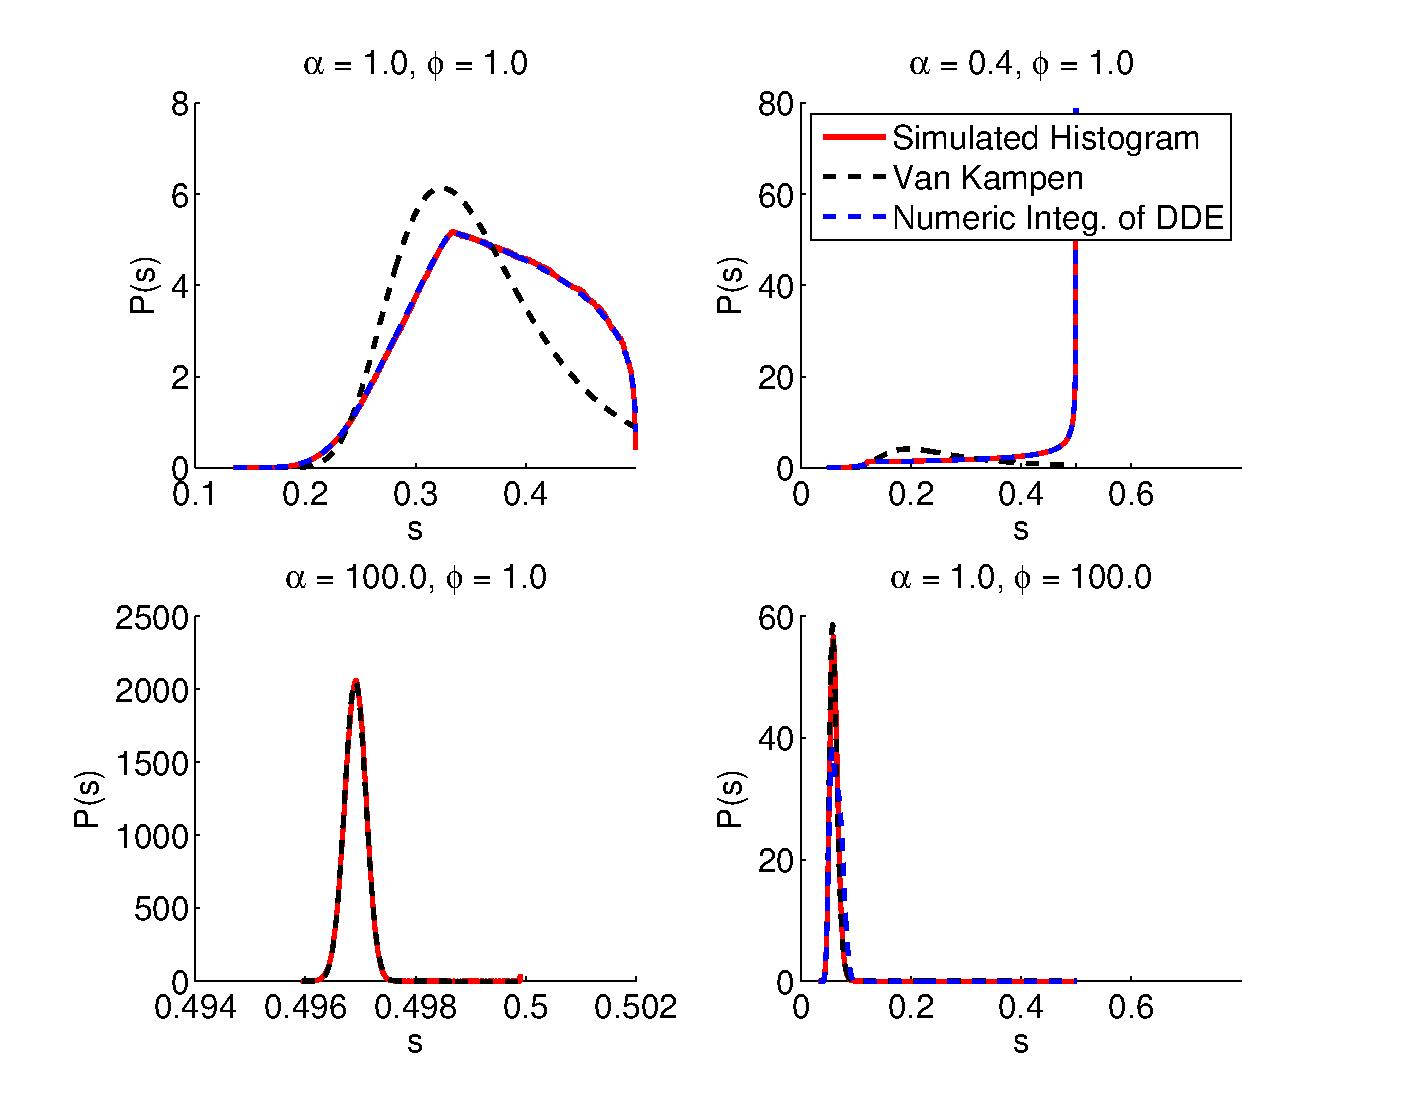
\includegraphics[width=\columnwidth]{figures/figure_3_1.eps}
\caption[Comparison of different solution approaches for the stationary distribution of variances.]{The two approaches to solving for the equilibrium distribution described, shown across a range of parameter values.}
\end{figure}
One particularly interesting characteristic of \fref{eq:dist_1d_exact} is its exponent. The sign of the exponent in \fref{eq:dist_1d_exact} depends on the specific value of $\hat{\lambda}$ 
and $2\gamma$. If $\hat{\lambda} > 2\gamma$, the exponent will be larger than 0, leading the distribution to tend to $0$ as $s$ tends to $s_0$. If, however, 
$\hat{\lambda} < 2\gamma$, the exponent will be negative, leading the distribution to diverge around $s_0$. Notice that $s_0$ is the worst possible performance our encoder can 
achieve, as it is the stationary variance of the unobserved process. This means that whenever the firing rate of the population is below a certain value, the probability distribution of our MSE will 
be dominated by its worst possible value. These results are illustrated in \fref{fig:comparison_histograms}. This is very interesting, as it relates two different time scales, 
one ($1/2\gamma$) describing how long information about the observed process stays relevant, the other ($1/\hat{\lambda}$) describing the average time between observations. It is 
intuitive to say that if the interval between spikes is much larger than the correlation time of
the process, one would expect estimation of the system's state to be bad. But here I have provided a simple analytic argument showing that, for a simple system
whenever the average inter spike interval is longer than the correlation time of the observed process, the mode of the distribution of errors will be the worst possible 
error for the estimator.
\par
Although the obtained distribution is always valid in the interval $S_0$, it can be shown to hold in the limit of low firing rates as well. This 
can be extended numerically to higher dimensions. Assuming the population firing rate $\hat{\lambda} \ll 2\gamma$, one will find that the expected interspike interval is much longer than the 
characteristic time of the variance's dynamics. It is then safe to assume, that whenever a spike is fired, the variance is very close to the stationary variance of the unobserved process 
$\Sigma_0 = \eta/2\gamma$. The 
evolution of it after the spike time $t_s$ will then be given by
\[
\Sigma(t) = e^{-2\gamma(t-t_s)} \Sigma' + \Sigma_0 \left(1-e^{-2\gamma (t-t_s)}\right),
\]
where $\Sigma' = j(\Sigma_0)$.
Solving for the time, one obtains
\[
\tau(\Sigma) \equiv (t-t_s) = -\frac{1}{2\gamma} \log\left(\frac{\Sigma_0-\Sigma}{\Sigma_0-\Sigma'}\right).
\]
Clearly, if the spikes are sampled from a Poisson process, then the interspike intervals have an exponential distribution $P(\tau) \propto e^{-\hat{\lambda}\tau}$. A change of 
variables thus leads to the density
\[
P(\Sigma) = P(\tau) \left|\frac{d\tau}{d\Sigma}\right| \propto e^{-\hat{\lambda} \tau + 2\gamma \tau}.
\]
Inserting the definition for $\tau$ one recovers \fref{eq:dist_1d_exact}. This is an approximation for $P(\Sigma)$ throughout the range of $s$ for a particular parameter limit, whereas before
I had derived an exact result for any parameters, but limited to a small range of values of $\Sigma$.\par

\subsection{An Extension to the Multidimensional Case}

I will derive a similar limit for the multidimensional case. First assume $\hat{\lambda}$ is small enough for the covariance $\Sigma$ to have relaxed to the stationary covariance of the unobserved process $\Sigma_0$. After a spike the covariance is then given by $\Sigma' = \left(\Sigma_0^{-1}+\covar^\dagger\right)^{-1}$. The evolution of $\Sigma(t)$ after a spike at $t_s$ is
\[
\Sigma(\tau) = e^{\tau A} \Sigma' e^{\tau A^\top} + \int_0^\tau e^{t A}\eta e^{t A^\top} dt.
\]
It is not possible to proceed as before, since the mapping from the matrix space of $\Sigma$ to the one-dimensional time space can not be explicitly written as above.
One could try to work out the densities for individual entries of the matrix $\Sigma$ but these would 
possibly not be one-to-one. One alternative is to evaluate the marginals of the matrix entries numerically through integration of the dynamics of $\Sigma(\tau)$.
One could thus integrate $\Sigma(t)$ numerically until it has reached the stationary value $\Sigma_0$, and evaluate the derivatives $\dot{\Sigma}$ numerically. This allows one to
look at the marginal probabilities of each entry of $\Sigma$, leading for example to
\[
P(\Sigma_{11}) = \frac{P(\tau(\Sigma_{11}))}{\left|\frac{d \Sigma_{11}}{d\tau}\right|} \propto \frac{e^{-\hat{\lambda} \tau}}{\left|\frac{d \Sigma_{11}}{d\tau}\right|},
\]
where $\tau(\Sigma_{11})$ is simply the time associated to that particular value of $\Sigma_{11}$ in the numerical integration.
If $A$ introduces interactions between the entries of the covariance matrix, however, this result will not prove as powerful. As an example, consider the Matern processes treated in \mycitep{Susemihl2013}, 
where the unobserved covariance evolves as
\begin{eqnarray*}
\frac{d\Sigma_{11}}{dt} = &2 \Sigma_{12},\\
\frac{d\Sigma_{12}}{dt} = \frac{d\Sigma_{21}}{dt} =& \Sigma_{22} -2 \gamma \Sigma_{11} -\gamma^2 \Sigma_{12},\\
\frac{d\Sigma_{22}}{dt} = & \eta -4 \gamma \Sigma_{12} -2\gamma^2\Sigma_{22}.
\end{eqnarray*}
The numerical approach for this Matern process is shown in \fref{fig:matern_histograms}, and again it coincides well with the distribution in the regime of low firing rates. It is important
to note, that because of the higher-order dynamical nature of the covariance, the divergence of $\Sigma_{11}$ around its stationary value no longer dominates the distribution, as
$\frac{d\Sigma_{11}}{dt}|_{\Sigma'} = 0$, leading to a second peak in the distribution around $\Sigma'_{11}$. 
%Furthermore, even in the limit of low firing rates, the effect of
%consecutive spikes can still be seen due to the slower relaxation of the covariance. This is given by the left side of the histogram in \fref{fig:matern_histograms}.

\begin{figure}
\label{fig:matern_histograms}
\includegraphics[width=\columnwidth]{figures/matern_histogram.eps}
\caption[Distribution of variances in the limit of small firing rates.]{The small firing rate limit for the Matern process.}
\end{figure}

\subsection{Van Kampen Approximation}

It is interesting to consider a different limiting behaviour to gain insight into the fluctuations of $\Sigma$. The Van Kampen approximation is a system size expansion, often
employed in the field of statistical physics. It consists of expanding the transition
probabilities around the deterministic solution in powers of the inverse system size and solving the dynamics of the resulting Focker-Planck equation. It is not evident how to choose
a system size for the problem at hand, but below I will show that it makes sense to consider the quantity $\gamma \alpha^2/\eta$ as a system size. It is simple to apply this
to the OU problem by taking the scaled inverse variance $z= \frac{\eta}{\gamma \Sigma}$ instead of the variance.
Note that although the change in the variance when a spike is observed is nonlinear, the change in the inverse variance is linear. This leads to the ODE
\[
\frac{dz}{dt} = -\gamma z \left(2- z\right) \textrm{ and the jump condition } z(t) = z(t^- ) + \frac{\eta}{\gamma \alpha^2}
\]
for all times $t$ when there is a spike observed. Defining the jump size as $\delta =  \frac{\eta}{\gamma \alpha^2}$, the differential Chapman-Kolmogorov equation for $P(z,t)$ is 
given by
\begin{equation}
\label{eq:DCKE_Z}
\frac{\partial P(z,t)}{\partial t} = \frac{\partial \left( \gamma z \left(2- z\right) P(z,t)\right)}{\partial z} + 
\hat{\lambda}\left[ P\left(z+\delta,t\right) - P(z,t)\right].
\end{equation}
The evolution of the average of $z$ is given by
\[
\frac{d \boldsymbol{E}\left[z\right]}{dt} = -\gamma\boldsymbol{E}\left[ z \left(2-z\right)\right]+ \hat{\lambda}\delta,
\]
which gives the mean-field stationary solution of $z^* =1+\sqrt{1+\hat{\lambda} \delta}$. 
This mean-field approach can be refined by expanding the nonlinear terms in \fref{eq:DCKE_Z} around $z^*$ up to first order, which will yield a linear Focker-Planck equation, which 
can be readily solved. The stationary solution to the Focker-Planck equation is a Gaussian distribution
\[
P_{eq}(z) = \mathcal{N}\left(\left(1+\sqrt{1+\hat{\lambda}\delta}\right), 
\frac{ \hat{\lambda}\delta^2 }{4\gamma \sqrt{1+\frac{\hat{\lambda}\delta}{\gamma} }}\right).
\]
With this solution in hand, it is easy to find the distribution of $\Sigma$ by a change of variables.
This approach is shown in \fref{fig:comparison_histograms} along with the numerical solution of the delayed-differential equation and the numerical simulations. 
Note that, again, \fref{eq:DCKE_Z} is still exact, and one can look at it to determine when the approximation is appropriate. I have Taylor expanded 
$P(z+\delta)$ keeping terms up to first order, and this will yield good approximations whenever $\frac{\eta}{\gamma\alpha^2}$ is small, that is, whenever the tuning width
is large compared to the stationary variance of the unobserved process. Furthermore, the nonlinear term $\gamma z (2-z)$ was also linearised around the mean-field stationary
value, which will only be a good approximation when $z$ has a small probability of wandering far from $z^*$. 
\par

In this case, $\frac{\gamma \alpha^2}{\eta}$ provides a system-size-like quantity for this system, giving us the order of magnitude of the fluctuations of the system. This can be understood
by noting that the change in $\Sigma$ after a jump is given by
$\Delta\Sigma = \frac{\Sigma^2}{\Sigma+\alpha^2}$. The jump can be treated as Gaussian noise if it is very small compared to the value of $\Sigma$, i.e.
\[
\frac{\Delta\Sigma}{\Sigma} = \frac{\Sigma^2}{\Sigma(\Sigma+\alpha^2)} = \frac{\Sigma}{\alpha^2} \frac{1}{1+\frac{\Sigma}{\alpha^2}},
\]
so the size of jumps relative to $\Sigma$ are of the order of $\Sigma/\alpha^2$ and can be safely treated as Gaussian noise if $\alpha^2$ is much larger than the typical value of 
$\Sigma$. $\Sigma$ is at most of the order of $\eta/2\gamma$ so the limit derived above makes sense. If $\gamma\alpha^2/\eta$ is very large, the fluctuations in $\Sigma$ should be 
small, rendering the Van Kampen approximation precise. This is seen to be the case in the lower left panel of
\fref{fig:comparison_histograms}, where the distribution of $\Sigma$ is narrow and the system size is large ($\gamma\alpha^2/\eta = 10000$), leading to a good agreement of the simulations with the 
Van Kampen approximation. In the lower right panel, the Van Kampen also fairs very well, but there the system size is 1. In the derivation above, however, I have used $\eta/\gamma$ as an upper
bound on values of $\Sigma$. As can be glanced from the histogram in the lower right of \fref{fig:comparison_histograms}, the typical value of $\Sigma$ is around $0.05$, due to the high firing rate.
So the actual system size as argued above would be of $\approx 50$, making the Van Kampen approximation justified.

\subsection{Prediction Error}
%Note that it is straightforward to derive 
What if I wanted to predict the value of the stimulus $X$ at a future time, for which I have no spike train information? In the absence of spikes the optimal MMSE estimator is given by 
the evolution of the mean and covariance with $dN^m(t) = 0$, and one would have the predictive probability
$P(X({t+\delta})|\{N^m_{0:t}\})$, with $\delta>0$. Here I am assuming the spikes are only observed up to time $t$, and I am trying to infer $X$ at some future time $t+\delta$.
The mean squared error or prediction error committed when estimating future values of $X$ in that way is given by
\begin{equation}
\boldsymbol{PE}_\delta(t) = \boldsymbol{E}_{X,\{N^m_{0:t}\}}\left[\left(X(t+\delta)-\mu(t+\delta;\{N^m_{0:t}\})\right)\left(X(t+\delta)-\mu(t+\delta;\{N^m_{0:t}\})\right)^\top\right].
\label{eq:C_delta}
\end{equation}
This gives us the matrix $\boldsymbol{MSE}$ when $\delta= 0$. For $\delta>0$ it gives the prediction error matrix.
Given a value of $X(t)$ and a realisation of the Wiener process $W(s)$ for $t\leq s \leq t+\delta$, one has
\[
X(t+\delta) = \int_0^{\delta} e^{-s A} \,H^{1/2} d W(s) + e^{-\delta A}\,X(t).
\]
Clearly, conditioning on $X(t)$ the above average is only over the Wiener process between $t$ and $t+\delta$. The estimator $\mu(t+\delta;\{N^m_{[0,t]}\})$ is also given by $\mu(t+\delta;\{N^m_{[0,t]}\}) = e^{-\delta A} \mu(t;\{N^m_{[0,t]}\})$ in the absence of spikes. The prediction error matrix will then be given by

\begin{eqnarray}
\boldsymbol{PE}_\delta(t)  =& \boldsymbol{E}_{W,\{N^m(0:t)\}}&\left[( \int_0^{\delta} e^{-(\delta-s)A} H d W(t+s) + e^{-\delta A}X(t)-e^{-\delta A}\mu(t))\times\right.\nonumber
\\
&&\left. (\int_0^{\delta} e^{-(\delta-u)A} H d W(t+u) + e^{-\delta A}X(t)-e^{-\delta A}\mu(t))^\top \right].\nonumber
\end{eqnarray}

Since $ e^{-(\delta-u)A} H$ is non-anticipating and does not depend on $X(t)$ or $N^m(t)$, one has that (see \mycitep{Gardiner2004})
$$
\boldsymbol{E}_{W}\left[\int_0^{\delta} e^{-(\delta-u)A} Hd W(t+u) \int_0^{\delta} e^{-(\delta-s)A} H dW(t+s))^\top \right] = \int_0^{\delta} e^{-(\delta-u)A}H^2 e^{-(t+\delta-u)A^\top} d u
$$
and therefore, changing variables,
\begin{equation}
\boldsymbol{PE}_\delta(t)= e^{-\delta A} \epsilon(t) e^{-\delta A^\top} + \int_{0}^\delta e^{-s A} H e^{-s A^\top}d s.
\label{eq:pred_error}
\end{equation}
This equation also describes the evolution of the variance of a linear stochastic processes,\footnote{See \citep[p.106]{Gardiner2004} for an example. This derivation is closely related to 
the derivation of the stationary variance for the OU process therein.} and it shows us that the prediction error is a simple function of the filtering error. This is also a consequence of the 
Markov nature of the posterior probability. Taking a non-Markov prior process would result in a posterior probability whose parameters could not be described by a finite set of ordinary 
differential equations.\par
\Fref{fig:prediction}  shows a comparison between the theoretical result in \fref{eq:pred_error} and simulation results for the prediction error. One can see that the prediction error is very well described by the derived equation.
\begin{figure}
\label{fig:prediction}
\includegraphics[width=.9\columnwidth]{figures/figure_3_3.eps}
\caption[Prediction Error.]{The evolution of the average prediction error $\mathcal{P}(\delta)$ is completely determined by the filtering error $\mathcal{P}(0)$. The blue line shows the prediction error obtained from the optimal filter in simulations, whereas the green line shows the evolution of the prediction error according to \fref{eq:pred_error} with the initial condition given by the average filtering error obtained in the simulations. The small discrepance between both curves is due to finite sample size effects.}
\end{figure}

\section{A Functional Approach to the MMSE}

\label{sec:kernels}

In \fref{sec:gp_filtering}, I have introduced Gaussian Process regression as a method of filtering general Gaussian Processes. So far, I have only considered stochastic processes
which are Markovian or can be rendered Markovian by an embedding into a higher-dimensional stochastic process.\footnote{See \fref{sec:stochastic_proc}} It is easy to adapt the
treatment given in \fref{sec:gp_filtering} to the case of Poisson processes. Say I am given a Gaussian process with zero mean and covariance function $K(s,v)$ and spike trains
from a dense population of Gauss-Poisson neurons. Assuming up to time $t$ there have been $M$ spikes, at times $\{t_i\}$ fired 
by neurons $\{n_i\}$ and the tuning centres of the spiking neurons are given by $\boldsymbol{\theta} = (\theta_{n_1}, \ldots, \theta_{n_M})^\top$, the posterior mean and covariance are
\begin{equation}
\mu(t) = k(t,\{t_i\})^\top (G + \alpha^2 \boldsymbol{I})^{-1} \boldsymbol{\theta},
\end{equation}
and
\begin{equation}
\Xi(t,t) =  K(t,t) - k(t,\{t_i\})^\top (G+\alpha^2\boldsymbol{I})^{-1} k(t,\{t_j\})^\top.
\end{equation}
Here $G_{i,j} = K(t_i,t_j)$ and $\alpha^2$ is the width of the tuning functions. The covariance of the posterior distribution at two
points is given by
\[
\Xi(s,t) = k(s,t) - \sum_{i,j} k(s,t_i) C_{ij} k(t_j,t).
\]
I will call the quantity $\Xi(s,t)$ the posterior kernel, as it again defines a GP. According to the formalism derived so far the MMSE for a filtering 
problem is simply the expected value of the posterior kernel $\Xi(t)$ averaged over the distribution of all possible past observations. Like I have done for the 
MMSE, I can look into the dynamics of the posterior kernel $\Xi(s,t)$. Defining $f_t(u,v) = \Xi(t+u,t+v)$, one has
\[
\frac{\partial f_t(u,v)}{\partial t} = \left( \frac{\partial }{\partial u}+ \frac{\partial }{\partial v}\right) f_t(u,v).
\]
It is a simple exercise in matrix inversion lemmas to show that, if a observation is obtained at time $t$ the posterior kernel will change as
\[
f_t(u,v) = f_{t^-}(u,v) - \frac{f_{t^-}(u,0)f_{t^-}(0,v)}{\alpha^2+ f_{t^-}(0,0)}.
\]
Taking the average over all possible observation paths one obtain the evolution of the average posterior kernel
\[
\frac{\partial \boldsymbol{E}\left[f_t(u,v)\right]}{\partial t} = \left( \frac{\partial }{\partial u}+ \frac{\partial }{\partial v}\right) \boldsymbol{E}\left[f_t(u,v)\right] - \hat{\lambda}\boldsymbol{E} \left[\frac{f_{t}(u,0)f_{t}(0,v)}{\alpha^2+ f_{t}(0,0)}\right].
\]
Again, I am most interested in the stationary case, so setting the derivative to zero one obtains
\begin{equation}
\label{eq:differential_kernel}
\left( \frac{\partial }{\partial u}+ \frac{\partial }{\partial v}\right) \boldsymbol{E}\left[f(u,v)\right] = \hat{\lambda} \boldsymbol{E}\left[\frac{f(u,0)f(0,v)}{\alpha^2+ f(0,0)}\right].
\end{equation}
Using the mean-field approximation leads to
\begin{equation}
\label{eq:kernel_mf}
\left( \frac{\partial }{\partial u}+ \frac{\partial }{\partial v}\right) \boldsymbol{E}\left[f(u,v)\right] = \hat{\lambda} \frac{ \boldsymbol{E}\left[f(u,0)\right]  \boldsymbol{E}\left[f(0,v)\right] }{\alpha^2+  \boldsymbol{E}\left[f(0,0)\right] }.
\end{equation}
This is solved by the integral equation
\begin{equation}
\label{eq:integral_kernel}
\boldsymbol{E}\left[f(u,v)\right] = k(u,v) - \frac{\hat{\lambda}}{\alpha^2+ \boldsymbol{E}\left[f(0,0)\right]} \int_0^\infty \boldsymbol{E}\left[f(s+u,0)\right]\boldsymbol{E}\left[f(0,s+v)\right] ds,
\end{equation}
as long as the kernel $k(u,v)$ is stationary, which implies $\partial_u k(u,v) = - \partial_v k(u,v)$.\footnote{A stationary kernel is such that 
$k(t,v) = k(\|t-v\|)$. If $t > v$ and $t> v+d$, then $k(t,v+d) = k(t-d,v)$. Differentiating with respect to $d$ we obtain the desired result.}\par

\Fref{eq:integral_kernel} allows one to approximate the shape of the posterior kernel directly from the prior kernel, without having to resort to the Markovian structure of
the process as we had done before. This is very convenient as it allows one to treat non-Markovian GP's such as the one defined by the squared exponential or Radial
Basis Function kernel.\footnote{The SE or RBF kernel is given by $k(t,v) = c \exp(-|t-v|^2/L^2)$.} This relies on the Mean-field approximation, but it is
still a very pleasing result, as it additionally allows one to estimate the shape of the entire posterior kernel, not only of the one-time variance. If one is only interested
in the filtering error however, it suffices to take the function $g(u) = \boldsymbol{E}\left[f(u,0)\right]$, where the filtering error is then given by $g(0)$. For that the equation simplifies to
\begin{equation}
\label{eq:integral_one_point}
g(u) = k(u,0)  - \frac{\hat{\lambda}}{\alpha^2+ g(0)} \int_0^\infty g(s+u)g(s) ds
\end{equation}
One way to solve \fref{eq:integral_one_point} is to simply discretise the real line over some interval $[0,D]$ and iterate \fref{eq:integral_one_point} numerically. I will discuss this approach shortly in \fref{app:kernel_integral}. This is shown in \fref{fig:integral_kernel} for the OU kernel $k_{OU}(s,t) = \exp(-|s-t|/k)$, for the Matern kernel $k_{mat}(s,t) = (1+\sqrt{3}|t-s|/k) \exp(-\sqrt{3}|t-s|/k)$ and the 
RBF kernel $k_{dbf} = \exp(-|t-s|^2/2k^2)$. As one moves towards smoother processes, the variance of the posterior kernel decreases, and the effect of the observations becomes more pronounced.

\begin{figure}
\label{fig:integral_kernel}
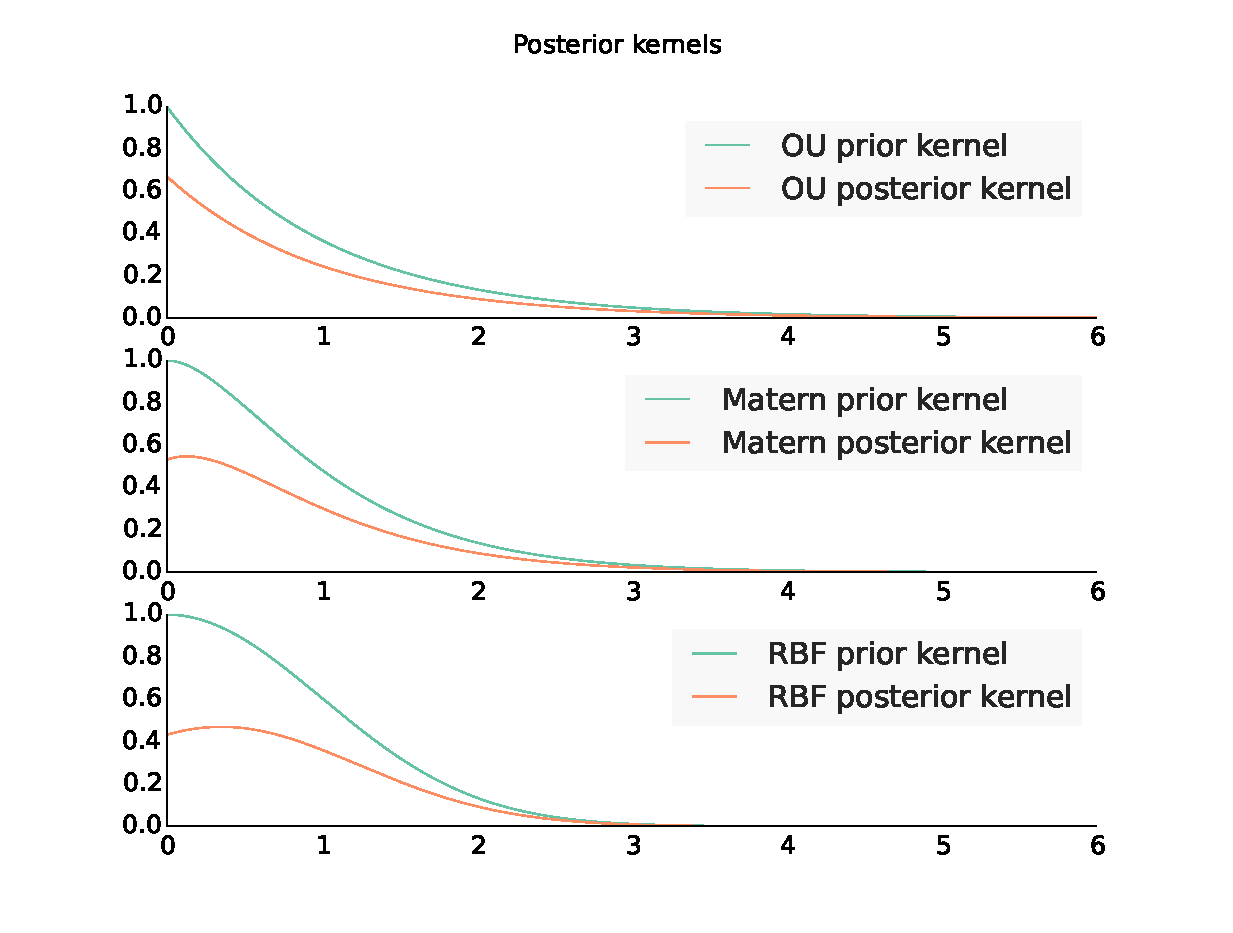
\includegraphics[width=\columnwidth]{figures/figure_3_4.eps}
\caption[Posterior kernels for general Gaussian processes]{The prior and posterior kernels for the filtering problem for three classes of GP's.}
\end{figure}

This can be used to study the MMSE of more complex Gaussian processes. The RBF kernel and the associated Gaussian process have been the subject of great
interest, specially in the Machine Learning community, as the squared exponential form of it often allows one to simplify a number of expressions in Gaussian
averages. Marc Deisenroth, for example, proposed to use the Gaussian form of the RBF kernel to average over uncertainty in the input $t$ of the process 
as
well as in the observation $Y$.\mycite{deisenroth2009} However, though it has proven very useful in ML, the RBF kernel is often criticised for being too smooth.\mycite{Rasmussen2005} 
A function $f(s)$ drawn from a GP with an RBF kernel is $\mathcal{C}^\infty$, leaving little room for randomness in its proper sense. On the other hand, \mycitet{Huys2007} have argued
that experimental trajectories of freely moving animals show an autocorrelation that is compatible with the RBF kernel. Though it might be a too strong prior to impose on natural 
stimuli, the RBF kernel might still be useful to model animal behaviour, with its longer time dependence.

\section{Alternative Performance Measures for Estimation}

I have chosen to focus on the mean-squared error of an estimation problem as a measure of efficiency of a neural population code. This is by no means the
only alternative there is. Many studies in computational neuroscience have focused on the Fisher information,\mycite{Ganguli2011,Zhang1999a,Brunel1998} and information-theoretical 
quantities such as the entropy or the mutual information of a code.\mycite{Schneidman2003,Tkacik2010,,Brunel1997} I will review the motivation and discuss the application of these tools in 
the present setting if merited.

\subsection{Fisher Information}
\label{sec:fisher_info}

The Fisher information gives an alternative measure to the amount of information carried by an observation $Y$ about an unobserved parameter or variable $x$.
The Fisher information $\mathcal{I}(x;Y)$ of $Y$ about $x$ is given by
\begin{equation}
\mathcal{J}(x;Y) \equiv \int P(Y|x) \left(\frac{\partial \log\left(P(Y|x)\right)}{\partial x}\right)^2 dY.
\end{equation}
Intuitively, the Fisher information tells one how sensitive the likelihood of an observation is to a change in the unobserved variable $x$ at that particular value. So,
a code that gives a high Fisher information on average will be very sensitive to changes in $x$, allowing for good estimation of $x$ from $Y$.
The relationship between estimation and the Fisher information can be made rigorous through the Cram\'{e}r-Rao bound. If one has an estimator
$\hat{x}(Y)$ of $x$ based on observations of $Y$, the Cram\'{e}r-Rao bound states that the variance of that estimator is bounded by
\begin{equation}
\label{eq:crb}
\boldsymbol{E}_{Y|x} \left[\left(\hat{x}(Y) - x\right)^2\right]  \ge \frac{\left(1+\frac{\partial b(x)}{\partial x}\right)^2}{\mathcal{J}(x;Y)},
\end{equation}
where $b(x) = \boldsymbol{E}_{Y|x}[\hat{x}(Y)] - x$ is the bias of the estimator. If $\hat{x}(Y)$ is unbiased this simplifies to
\[
\boldsymbol{E}_{Y|x} \left[(\hat{x}(Y) -x)^2\right]  \ge \frac{1}{\mathcal{J}(x;Y)}.
\]
In the multivariate case this becomes a restriction on the positive-definiteness of the MSE matrix, more precisely, for the unbiased case, one has that for any
$v$ it holds that 
\[
v^\top \boldsymbol{E}_{Y|x} \left[(\hat{x}(Y) -x)(\hat{x}(Y) -x)^\top\right] v \ge v^\top \mathcal{J}(x;Y)^{-1} v,
\]
which means that the matrix $\boldsymbol{E}_{Y|x} \left[(\hat{x}(Y) -x)(\hat{x}(Y) -x)^\top\right]-\mathcal{J}(x;Y)^{-1}$ is positive semidefinite.\par

The Cram\'{e}r-Rao bound can also be extended to a Bayesian setting, where one is no longer estimating a fixed parameter but a random variable. Considering $X$
a random variable with distribution $P(X)$, one obtains the Bayesian Cram\'{e}r-Rao Bound (BCRB),
\[
\boldsymbol{E}_{X,Y} \left[\left(\hat{X}(Y) - X\right)^2\right]  \ge \frac{1}{\boldsymbol{E}_X\left[\mathcal{J}(X;Y)\right] + \mathcal{I}(X)},
\]
where
\[
\mathcal{I}(X) = \int dX P(X) \left(\frac{\partial \log P(X)}{\partial X}\right)^2.
\]
Unlike the Cram\'{e}r-Rao Bound given in \fref{eq:crb}, the BCRB gives a bound on the performance of a given code in an environment regardless of the 
system's state.\par

The Fisher information is particularly popular in the neuroscience community partly because it has a convenient form for rate-based models. Suppose one has a Poisson neuron
with some tuning function $f(X)$. The probability of a spike count $r$ in a time interval of duration $T$ is given by
\[
P(r|X) = \frac{e^{-T f(X)T}(T f(X))^r}{r!}, \quad \log(P(r|X)) = r \log (T f(X)) - T f(X) - \log r!.
\]
This leads to the Fisher information
\[
\mathcal{J}_{Poiss} (X;Y) = T \frac{f'(X)^2}{f(X)} = \frac{(T f'(X))^2}{T f(X)},
\]
which is a function of $T f(X)$, the expected number of spikes for the experiment. In \fref{fig:fisher_info} I have shown the Fisher
information for a Gaussian tuning function as a function of $X$.

\begin{figure}
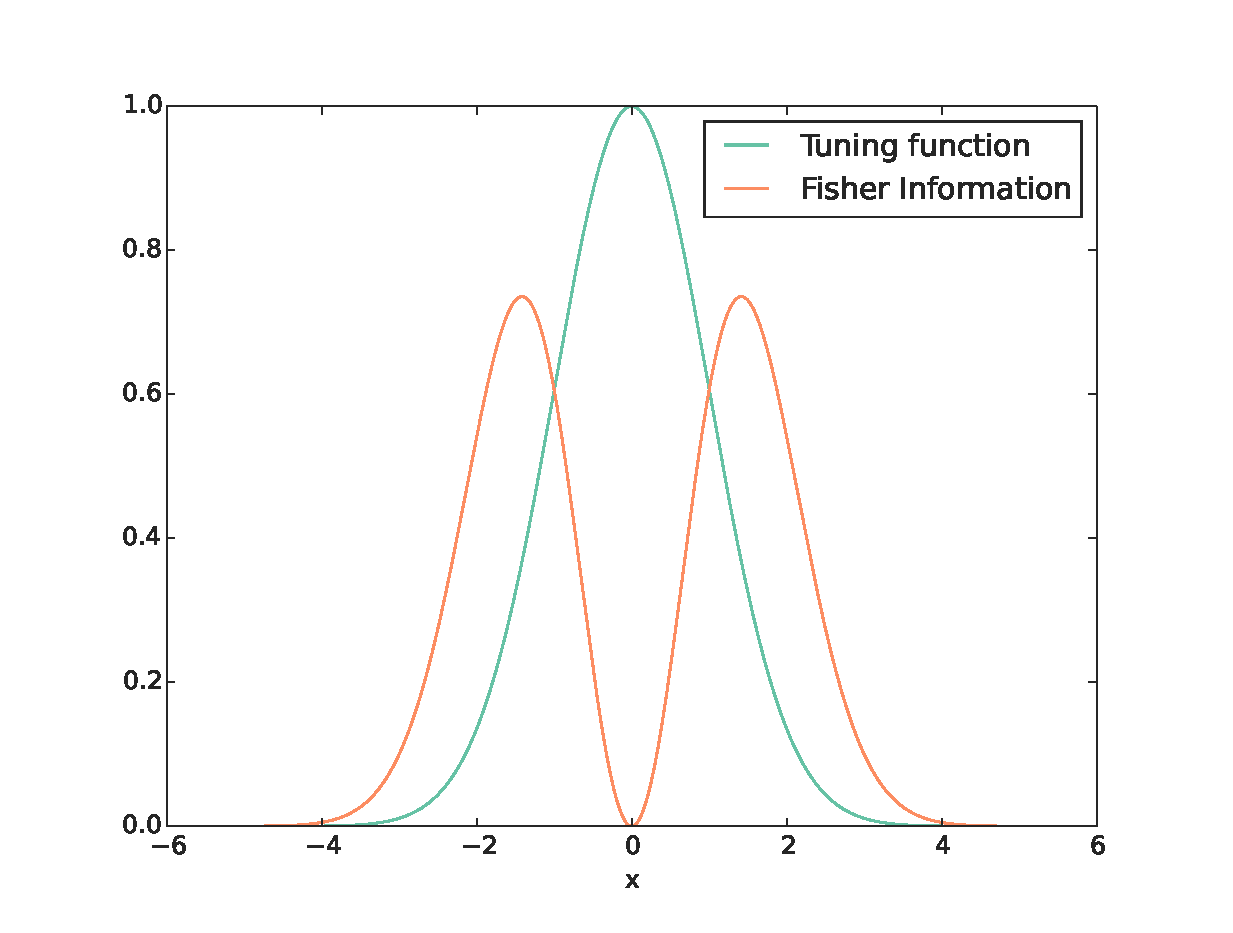
\includegraphics[width=\columnwidth]{figures/figure_3_5.eps}
\caption[Fisher Information for a Gauss-Poisson neuron.]{The Fisher information of a Gaussian-shaped tuning function. Note how the information is highest around the slopes of the tuning function. This approach
puts a higher prize on discriminability, so the highest information is achieved when the slope of the tuning function is highest.}
\label{fig:fisher_info}
\end{figure}

\par
One can see why this is of interest for
computational neuroscientists, as rate-based models are the bread and butter of spike train analysis. A number of experiments sought to use the Fisher information
as a measure of performance for coding strategies, such as \mycitep{Zhang1999a,Brunel1998} for example. More recently, this line of reasoning has been criticised
by a number of findings. Matthias Bethge, for example, argued that the Cram\'{e}r-Rao bound is loose in general and only provides a tight bound on the MMSE of a
neural population code in the limit of very long times and many spikes, rendering it of limited usability.\mycite{Bethge2002} For the dynamic setting I am considering,
where the dynamic nature of the stimulus is central, Fisher information seems to be of little use. \mycitep{Yaeli2010} and \mycitep{Berens2011} have compared the MMSE with
the Cr\'{a}mer-Rao bound extensively, coming repeatedly to the conclusion that the Cr\'{a}mer-Rao bound leads to troubling results, such as the optimal
code not depending on the decoding time available. I will therefore not spend any further time investigating the Fisher information in this thesis.

\subsection{Mutual Information}
\label{sec:mutual_info}

The canonical tool to quantify the level of dependence between two variables in information theory is the mutual information. Though the correlation is often 
preferred, the mutual information provides the guarantee that it is zero if and only if the random variables are statistically independent, providing a way of robustly quantifying the level 
of dependence between two variables. The mutual information was defined in \fref{chap:intro} as
\[
I(X;Y) = \int dX dY P(X,Y) \log \left(\frac{P(X,Y)}{P(X)P(Y)} \right),
\]
which can be readily cast into
\[
I(X;Y) = \int dX dY P(Y) P(X|Y) \log \left(\frac{P(X|Y)}{P(X)} \right) = \boldsymbol{E}_Y \left[H(X) - H(X|Y)\right],
\]
which gives the average reduction of entropy in $X$ upon observing a random value of $Y$.  One advantage of the mutual information is that it does not make
any reference to an estimator or a reconstruction procedure, giving us a principled quantification of the information obtained about one variable from an observation
of the other. The main disadvantage of the mutual information is that it is much harder to compute than other quantities, as one is required to estimate the whole
probability distribution of $X$ and $Y$ to do so.\par

Another important issue one should note, is that the interpretation of the mutual information as an reduction of the entropy is more problematic in the continuous case. As I had noted 
before, the differential entropy can given negative values, making the last step of the equation above a bit delicate. Furthermore, the mutual information between two continuous 
random variables is only defined if their densities are absolutely continuous with respect to each other. In the sense of probability theory, this means that the mutual information is only
defined if, whenever $P(X,Y) > 0$ then $P(X)P(Y) > 0$. The probability densities I am considering here are mostly Gaussian, and therefore positive through their whole domain, so
this will not be an issue in the present case.\par

More recently, there have also been a number of results relating the mutual information to the MMSE of estimators. One of the most surprising results is probably is that for an additive
Gaussian channel, where one is trying to estimate the value of a random variable $X$ from an observation of $Y = k^{1/2} X + N$, the following relationship holds
\[
\frac{\partial I(X;Y)}{\partial k} = \frac{1}{2} MMSE(\hat{X}(Y)).
\]
This holds regardless of the distribution of the random variable $X$.
This is one of the so-called I-MMSE relations, which have been a very popular area of study in the field of information theory recently.\mycite{guo2005,wu2010,merhav2011}

For the dense Gauss-Poisson populations under consideration one can evaluate the mutual information readily. Assume that at time 0, knowledge of the
system's state $X$ is given by some normal distribution $P_0(X)$. One can then easily evaluate the mutual information of the system's
state at time $t$, $X(t)$ and the spike train up to time $t$, $N_{0:t}$. To that end, one needs only to note that the marginal $P(X(t))$ is given by a Gaussian with
moments evolving according to \fref{eq:free_ou_moments}, which I will denote as $\mu^0(t)$ and $\Sigma^0(t)$. The posterior distribution is given simply
by the solution of the filtering equations for the problem. The distributions are given by
\[
P(X(t)) = \mathcal{N}(\mu^0(t),\Sigma^0(t)), \textrm{ and } P(X(t) | N_{0:t}) = \mathcal{N}(\mu(t; N_{0:t}), \Sigma(t; N_{0:t})),
\]
and therefore
\[
I(X(t);N_{N_{0:t}}) = \log |\Sigma^0(t)| - \boldsymbol{E}_{N_{0:t}}\left[\log |\Sigma(t; N_{0:t})|\right].
\]
Here again, one is faced with an average over $P(\Sigma,t)$, this time of the logarithm of the determinant of $\Sigma(t)$. In the mean-field approximation, this will give simply the
logarithm of the determinant of the matrix $\epsilon(t)$. I will show in \fref{chap:optimal} that the mutual information leads to the same optimal codes as the MMSE for the OU process.

